\documentclass{article}
\usepackage{tikz}
\usetikzlibrary{shapes, arrows.meta, positioning, shapes.geometric}
\usepackage{amsmath}
\usepackage{amssymb}
\tikzstyle{process} = [rectangle, 
minimum width=1.5cm, 
minimum height=0.8cm, 
text centered, 
text width=2cm, 
draw=black, 
fill=orange!30]

\tikzstyle{decision} = [diamond, 
minimum width=1.5cm, 
minimum height=0.8cm, 
text centered, 
draw=black, 
fill=green!30]
\tikzset{
    %process/.style = {rectangle, draw, text width=6em, text centered, minimum height=1.5em},
    %decision/.style = {diamond, draw, text width=5.5em, text centered, aspect=2, minimum height=1.5em},
    answer/.style = {rectangle, draw, text width=2em, text centered, minimum height=1em, fill=gray!20},
    arrow/.style = {thick, -Stealth}
}

\begin{document}
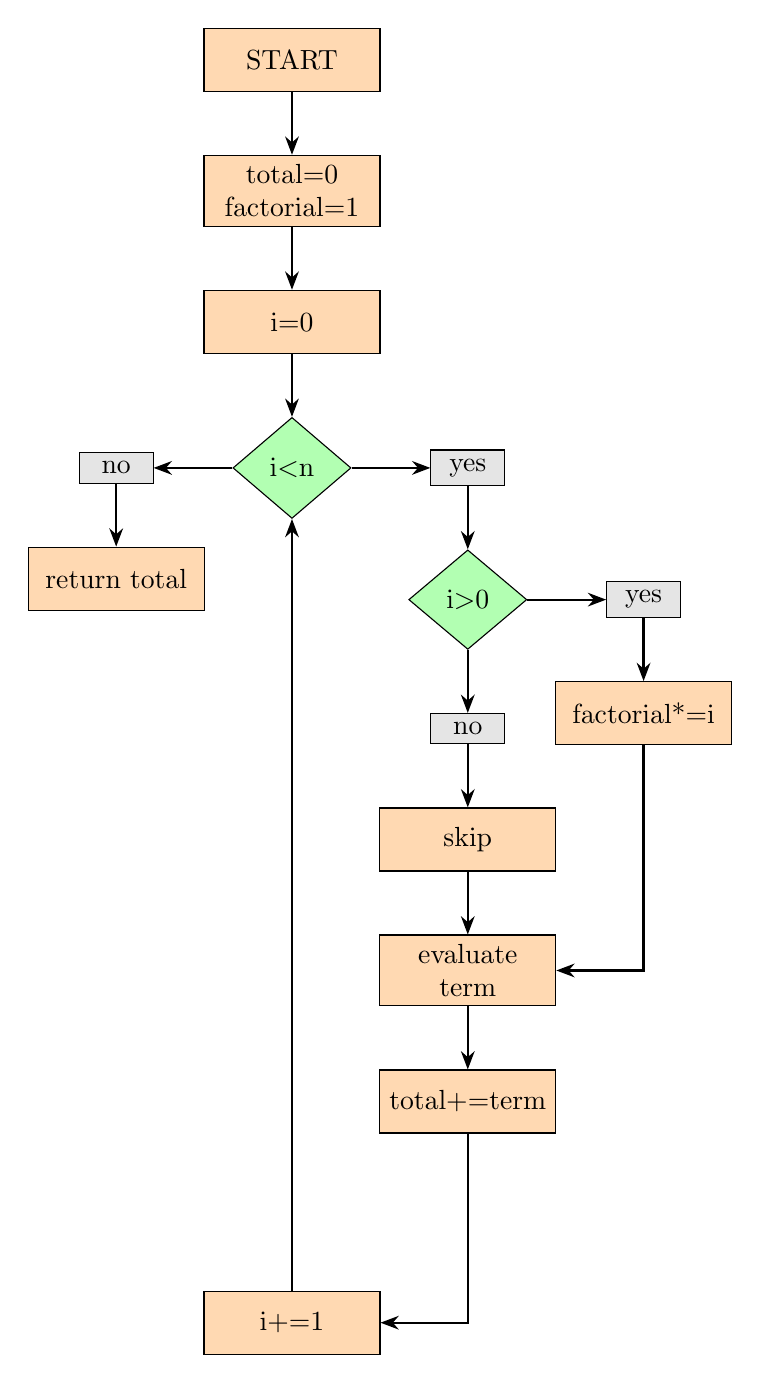
\begin{tikzpicture}[xshift={(-3cm)}, node distance=0.8cm and 1cm]
%Nodes 
\node (process0) [process] {START};
\node (process) [process, below=of process0] {total=0 factorial=1};
\node (process1) [process, below=of process] {i=0};
\node (decision) [decision, below=of process1] {i\textless n};
\node (no1) [answer, left =of decision] {no};
\node (process6) [process, below=of no1] {return total};
\node (yes1) [answer, right =of decision] {yes};
\node (decision2) [decision, below=of yes1] {i\textgreater 0};
\node (no2) [answer, below =of decision2] {no};
\node (yes2) [answer, right =of decision2] {yes};
\node (process2) [process, below=of no2] {skip};
\node (process7) [process, below=of yes2] {factorial*=i};
\node (process3) [process, below=of process2] {evaluate term};
\node (process4) [process, below=of process3] {total+=term};
\node (process5) [process, below=of decision, yshift=-9cm] {i+=1};




%ARrrows
\draw [arrow] (process0) -- (process);
\draw [arrow] (process) -- (process1);
\draw [arrow] (decision) -- (yes1);
\draw [arrow] (process1) -- (decision);
\draw [arrow] (decision) -- (no1);
\draw [arrow] (no1) -- (process6);
\draw [arrow] (process2) -- (process3);
\draw [arrow] (process3) -- (process4);
\draw [arrow] (process4) |- (process5);
\draw [arrow] (yes1) -- (decision2);
\draw [arrow] (decision2) -- (no2);
\draw [arrow] (no2) -- (process2);
\draw [arrow] (decision2) -- (yes2);
\draw [arrow] (yes2) -- (process7);
\draw [arrow] (process7) |- (process3);
\draw [arrow] (process5) -- (decision);

\end{tikzpicture}
\end{document}